\documentclass[12pt]{report}
\usepackage[utf8]{inputenc}
\usepackage[russian]{babel}
\usepackage{setspace} % для междустрочного интервала
\onehalfspacing % 1.5 интервал между строками

\usepackage[left=30mm, top=20mm, right=20mm, bottom=20mm, nohead, footskip=7mm]{geometry}

\usepackage{titlesec, blindtext, color} 
\definecolor{gray75}{gray}{0.75}
\newcommand{\hsp}{\hspace{20pt}}
\titleformat{\chapter}[hang]{\Large\bfseries}{\thechapter{. }}{0pt}{\Large\bfseries}
\titlespacing{\chapter}{-5pt}{-30pt}{12pt} % отступ заголовка сверху
\titleformat{\section}[hang]{\large\bfseries}{\thesection{. }}{0pt}{\large\bfseries}

\makeatletter % список литературы
\def\@biblabel#1{#1. }
\makeatother

% Ссылки
\usepackage{hyperref}

% Возможность вставки pdf страниц
\usepackage{pdfpages}

% Листинги
\usepackage{listings}

\lstset{
	language = c++,
	extendedchars=\true,
	basicstyle=\small\sffamily,
	numbers=left,
	numberstyle=\tiny,
	stepnumber=1,
	numbersep=5pt,
	showspaces=false,            % показывать или нет пробелы специальными отступами
	showstringspaces=false,
	showtabs=false,
	frame=single,
	tabsize=2,
	captionpos=t,
	breaklines=true,
	breakatwhitespace=false,
	escapeinside={\#*}{*)},
	keepspaces=true
}

% Чтобы вместо : в подписях было -
\RequirePackage{caption}
\DeclareCaptionLabelSeparator{defffis}{ — }
\captionsetup{justification=centering,labelsep=defffis}

\usepackage{pgfplots}
\usepackage{pgfplotstable}
\pgfplotsset{compat=1.9}

\usepackage{longtable}


\begin{document}
	\renewcommand\bibname{Список литературы}
	
	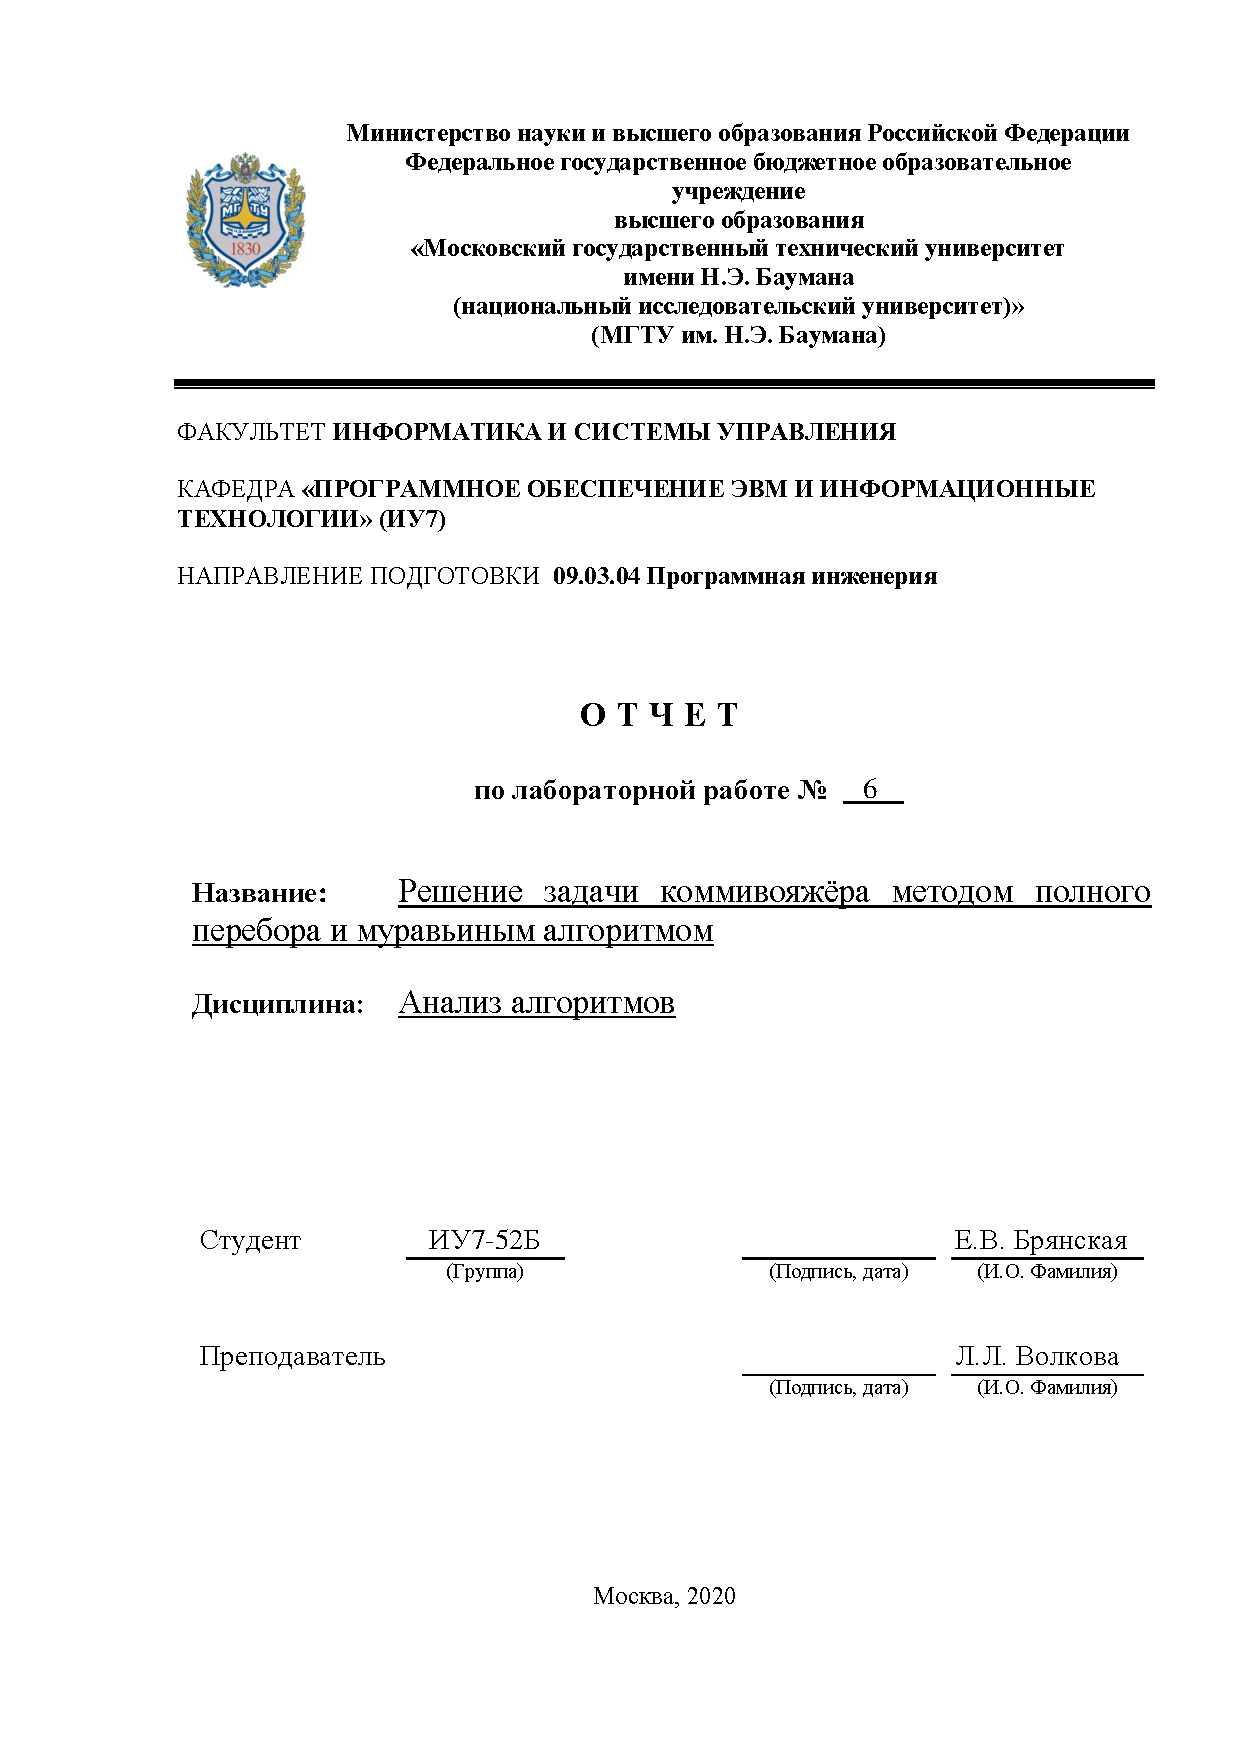
\includepdf[pages=1]{title.pdf}
	
	\tableofcontents
	\newpage
	
	\chapter*{Введение}
	\addcontentsline{toc}{chapter}{Введение}
	\textbf{Трудоёмкость алгоритма} - это зависимость стоимости операций от линейного(ых) размера(ов) входа(ов) \cite{labor_int}.\\

Модель вычислений трудоёмкости должна учитывать следующие оценки.
\begin{itemize}
	\item[1)] Стоимость базовых операций. К ним относятся: =, +, -, *, /, ==, !=, <, <=, >, >=, \%, +=, -=, *=, /=, [ ], < <, > >. Каждая из операций имеет стоимость равную 1.
	\item[2)] Оценка цикла. Она складывается из стоимости тела, инкремента и сравнения. 
	\item[3)] Оценка условного оператора if. Положим, что стоимость перехода к одной из веток равной 0. В таком случае, общая стоимость складывается из подсчета условия и рассмотрения худшего и лучшего случаев.
\end{itemize}

Оценка характера трудоёмкости даётся по наиболее быстрорастущему слагаемому.\\

\textbf{Сортировка} - процесс перегруппировки заданного множества объектов в некотором определенном порядке. Сортировка предпринимается для того, чтобы облегчить последующий поиск элементов в отсортированном множестве.\\

В этой лабораторной работе будет оцениваться трудоёмкость алгоритмов сортировки.
Будут рассмотрены следующие алгоритмы:
\begin{itemize}
	\item[1)] сортировка пузырьком;
	\item[2)] сортировка вставками;
	\item[3)] *****
\end{itemize}
	\newpage
	
	\chapter{Аналитическая часть}
	В этом разделе будут поставлены цель и основные задачи лабораторной работы, которые будут решаться в ходе её выполнения.

\section{Цель и задачи}
\qquad\textbf{Цель} данной работы: получить навык разработки конвейера, работающего в параллельном режиме.\\

Для достижения поставленной цели необходимо решить ряд следующих \textbf{задач}:
\begin{enumerate}
	\item[1)] описать алгоритмы, на основе которых будет строиться работа конвейера;
	\item[2)] описать алгоритм работы конвейера;
	\item[3)] реализовать все рассмотренные алгоритмы;
	\item[4)] получить время ожидания в очереди и полное время решения для каждой задачи;
	\item[5)] среди найденных временных значений найти минимальное/максимальное/среднее время.
\end{enumerate}

В качестве основной работы берётся шифрование строк, которое разделено на три стадии, на каждой из которых представлен свой алгоритм.

\section{Основные требования к алгоритмам шифрования}
Сюда нужно отнести следующее.
\begin{itemize}
	\item Алгоритм должен быть надёжным, не допускать ситуации, когда ключ (если он используется) и сам принцип шифрования успешно угадывались сторонними лицами.
	\item Должен допускать эффективную программную реализацию.
	\item И быть достаточно простым для написания кода, чтобы минимизировать вероятность программных ошибок.
	\item Если алгоритм использует ключи, то любую случайную строку битов нужной длины, следует рассматривать в качестве возможного ключа.
	\item Используемый метод должен легко модифицироваться для различных уровней безопасности и удовлетворять как минимальным, так и максимальным требованиям.
\end{itemize}

\section{Используемые алгоритмы шифрования}

\subsection{Алгоритм, в основе которого лежит операция XOR}
\qquadОдин из самых простых алгоритмов шифрования. Он основан на применении бинарной логической операции исключающего или (XOR). \\

Операция XOR обладает симметричностью. Это значит, что если зашифровать одну и ту же строку 2 раза с одним и тем же ключом, то в результате получается эта же строка без изменений.

\subsection{Шифр Виженера}
\qquadЭтот метод используется для шифрования буквенного текста с использованием ключевого слова. В его основе лежит алгоритм Цезаря, но в отличие от него, он более надежный и безопасный. \\

Шифр можно записать с помощью формулы \ref{formula1}.
\begin{equation}\label{formula1}
	c_i = (m_i + k_i)\:mod\:n,
\end{equation}
где $m_i$ -- код $i-$ой буквы строки, которую нужно зашифровать, $k_i$ -- код буквы ключа, $n$ -- количество букв в алфавите, $c_i$ -- итоговое значение кода зашифрованной буквы, $mod$ -- операция получения остатка от деления. Далее по коду символа определяется соответсвующая ему буква \cite{cript}.

\subsection{Транспозиция}
\qquadЭтот алгоритм основан на перестановке символов в строке по какому-либо правилу. Для усложнения метода используется двойная перестановка, т.е. после первого прохода по строке, осуществляется второй проход, также меняющий местами символы, но уже по другому принципу.\\

Таким образом, не зная правил, по которым производилось шифрование достаточно сложно подобрать нужные. Задача усложняется тем, что неизвестно сколько и какие методы используются в конкретном случае \cite{cript2}

\section{Общие принципы работы конвейера}
\qquadПусть конвейер состоит из трёх лент. Тогда будем симулировать каждую из них, потоком, причём, на каждую ленту выделено по одному потоку.
Под потоком подразумевается непрерывнная часть кода процесса, которая может выполняться с другими частями выполняемой программы.\\

Пусть существует план -- обработать N объектов. Рабочий поток живёт до тех пор, пока не выполнит весь план.\\

Главный поток запускает рабочие потоки и выдаёт задачи (объекты) на обработку первому потоку. После того, как задача обработается на первой ленте, она передаётся на вторую, в это время как, на первую поступает другая задача. Аналогично организуется работа на втором и третьем потоках. Процессы на лентах выполняются параллельно.\\

Когда все задачи будут последовательно обработаны на трёх лентах конвейера, главный поток соберёт статистику и выведет её в интерфейс, либо файл.\\

Перед тем, как пройти стадию обработки на какой-либо ленте, каждая задача попадает в очередь из таких же задач. Максимально полезная работа контейенера возникает тогда, когда загружены все потоки, и время простоя минимально.

\section*{Вывод}
\addcontentsline{toc}{section}{Вывод}
\qquadБыл рассмотрен общий принцип работы конвейера, а также алгоритмы шифрования на каждой из его лент.
	\newpage
	
	\chapter{Конструкторская часть}
	Рассмотрим выбранные алгоритмы сортировки. Для упрощения задачи будем сортировать последовательность по неубыванию. 
\section{Сортировка пузырьком}
\qquadОсуществляется проход по массиву от начала до конца, в процессе меняя местами неотсортированные соседние элементы.

В результате первого прохода на последнем месте окажется максимальный элемент. Далее снова делается проход по неотсортированной части массива (от первого до предпоследнего) и так же меняются неупорядоченные соседние элементы. Таким образом, на предпоследнее место будет помещён второй по величине элемент.

Действия повторяются до тех пор, пока не обработается вся неотсортированная часть. \\

\textbf{Схема} алгоритма представлена на Рис.\ref{fig1:image}.
%\begin{figure}[h]
%	\begin{center}
%		{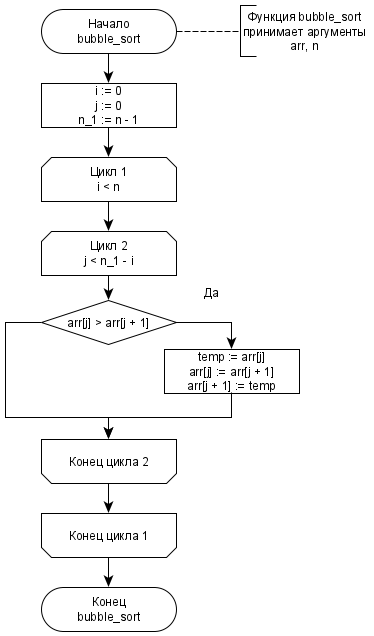
\includegraphics[scale = 0.46]{schemes/bubble}}
%		\caption{Сортировка пузырьком}
%		\label{fig1:image}
%	\end{center}
%\end{figure}

\section{Сортировка вставками}
\qquadВ этом алгоритме рассматриваемый массив условно делится на две части: отсортированная и нет. 

В начале работы отсортированной частью считается нулевой элемент. Далее берётся каждый следующий и сравнивается с уже отсортированной частью. Находится подходящая для текущего элемента позиция в ней, осуществляется сдвиг уже отсортированных элементов, но больших по величине, чем рассматриваемый. И затем рассматриваемый элемент помещается на найденную позицию.

И так до тех пор, пока не просмотрится вся неотсортированная часть.\\ 

\textbf{Схема} алгоритма представлена на Рис.\ref{fig2:image}.
%\begin{figure}[h]
%	\begin{center}
%		{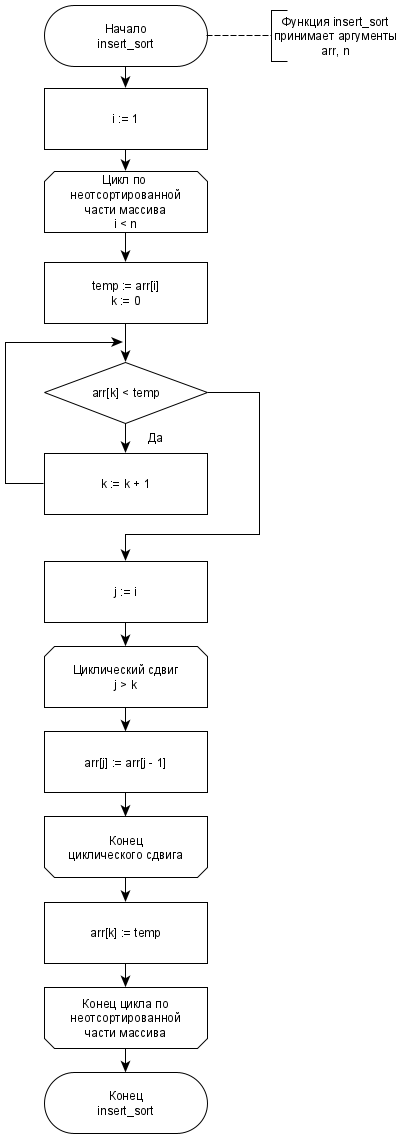
\includegraphics[scale = 0.46]{schemes/insert}}
%		\caption{Сортировка вставками}
%		\label{fig2:image}
%	\end{center}
%\end{figure}

\section{Поразрядная сортировка}
\qquadПроизводится сортировка массива целых положительных чисел, а также чисел, которые можно преобразовать в неотрицательные, путём увеличения всех элементов на величину, по модулю равную минимальному элементу.\\

Перед началом работы алгоритма находится максимальное количество разрядов $k$ среди рассматриваемых чисел.\\

Далее сравнение производится поразрядно: сначала рассматриваются значения одного крайнего разряда, и формируются группы элементов по результатам этого сравнения, затем сравниваются значения следующего соседнего разряда, и происходит переупорядочивание элементов по результатам текущего сравнения (с сохранением относительного порядка, который был достигнут ранее). Сравнения продолжаются до тех пор, пока не обработается $k$ый разряд.\\

\textbf{Схема} алгоритма представлена на Рис.\ref{fig3:image}.
%\begin{figure}[h]
%	\begin{center}
%		{\includegraphics[scale = 0.46]{schemes/lsd}}
%		\caption{Сортировка вставками}
%		\label{fig3:image}
%	\end{center}
%\end{figure}

\section{Требования к ПО}
\qquadДля корректной работы алгоритмов и проведения тестов необходимо выполнить следующее.
\begin{itemize}
	\item Обеспечить возможность ввода массива через консоль и выбора алгоритма сортировки.
	\item В случае ввода некорректных данных вывести соответствующее сообщение. Программа не должна аварийно завершаться.
	\item Программа должна отсортировать массив и вывести результат на экран.
	\item Реулизовать функцию замера процессорного времени, которое выбранный метод затрачивает на вычисление результатов. Для этого дать возможность ввода размера тестируемого массива. Вывести результаты замеров на экран.
\end{itemize}

\section{Заготовки тестов}
\qquadПри проверке на корректность работы реализованных функций необходимо провести следующие тесты:
\begin{itemize}
	\item отсортировать массив размером в один элемент;
	\item простой массив ненулевой длины;
	\item упорядоченный по невозрастанию массив;
	\item упорядоченный по неубыванию массив;
	\item массив, состоящий из одинаковых элементов.
\end{itemize}

	\newpage
	
	\chapter{Технологическая часть}
	\section{Выбранный язык программирования}
\qquadДля выполнения этой лабораторной работы был выбран язык программирования C++, так как есть большой навык работы с ним и с подключаемыми библиотеками, которые также использовались для проведения тестирования и замеров.\\

Использованная среда разработки - Visual Studio.

\section{Листинг кода}
\qquadНиже представлены Листиги 3.1 - 3.3 функций, реализующих алгоритмы поиска расстояний.
\begin{lstlisting}[label=code, caption = Стандартный алгоритм умножения матриц]
	matrix_t standart_mult(matrix_t a, matrix_t b, int m, int n, int q)
	{
		matrix_t c = create_matrix(m, q);
		
		for (int i = 0; i < m; i++)
			for (int j = 0; j < q; j++)
			{
				c[i][j] = 0;
				for (int k = 0; k < n; k++)
					c[i][j] += a[i][k] * b[k][j];
			}
		
		return c;
	}
\end{lstlisting}

\begin{lstlisting}[label=code, caption = Алгоритм Винограда]
matrix_t winograd_mult(matrix_t a, matrix_t b, int m, int n, int q)
{
	arr_t mulH = create_array(m);
	arr_t mulV = create_array(q);
	matrix_t c = create_matrix(m, q);
	
	for (int i = 0; i < m; i++)
	{
		mulH[i] = 0;
		for (int k = 0; k < n / 2; k++)
			mulH[i] = mulH[i] + a[i][2 * k] * a[i][2 * k + 1];
	}
	
	for (int i = 0; i < q; i++)
	{
		mulV[i] = 0;
		for (int k = 0; k < n / 2; k++)
			
			mulV[i] = mulV[i] + b[2 * k][i] * b[2 * k + 1][i];
	}
	
	for (int i = 0; i < m; i++)
		for (int j = 0; j < q; j++)
		{
			c[i][j] = -mulH[i] - mulV[j];
			for (int k = 0; k < n / 2; k++)
				c[i][j] = c[i][j] + (a[i][2 * k] + b[2 * k + 1][j]) * 
						  		(a[i][2 * k + 1] + b[2 * k][j]);
		}
	
	if (n % 2)
		for (int i = 0; i < m; i++)
			for (int j = 0; j < q; j++)
				c[i][j] = c[i][j] + a[i][n - 1] * b[n - 1][j];
	
	return c;
}
\end{lstlisting}

\begin{lstlisting}[label=code, caption = Оптимизированный алгоритм Винограда]
matrix_t winograd_mult(matrix_t a, matrix_t b, int m, int n, int q)
{
	arr_t mulH = create_array(m);
	arr_t mulV = create_array(q);
	double buf;
	
	matrix_t c = create_matrix(m, q);
	
	for (int i = 0; i < m; i++)
	{
		buf = 0;
		for (int k = 1; k < n; k += 2)
			buf += a[i][k] * a[i][k - 1];
		mulH[i] = buf;
	}
	
	for (int i = 0; i < q; i++)
	{
		buf = 0;
		for (int k = 1; k < n; k += 2)
			buf += b[k][i] * b[k - 1][i];
		mulV[i] = buf;
	}
	
	int temp = n - 1;
	int is_odd = n % 2;
	
	for (int i = 0; i < m; i++)
		for (int j = 0; j < q; j++)
		{
			buf = -(mulH[i] + mulV[j]);
			for (int k = 1, t = 0; k < n; k += 2, t +=2)
				buf += (a[i][k] + b[t][j]) * (a[i][t] + b[k][j]);
			c[i][j] = buf;
			
			if (is_odd)
				c[i][j] += a[i][temp] * b[temp][j];
		}
	
	return c;
}
\end{lstlisting}

\section{Результаты тестов}
\qquadДля тестирования были написаны функции, проверяющие, согласно заготовкам выше, случаи. Выводы о корректности работы делаются на основе сравнения результатов.

\textbf{Все тесты пройдены успешно.} Сами тесты представлены ниже (Листинг 3.4).\\

\begin{lstlisting}[label=code, caption = Тесты]
bool mult_cmp(matrix_t a, matrix_t b, int m, int n, int q)
{
	matrix_t c1 = standart_mult(a, b, m, n, q);
	matrix_t c2 = winograd_mult(a, b, m, n, q);
	
	bool res = cmp_matrix(c1, c2, m, q);
	
	free_matrix(&c1, m, q);
	free_matrix(&c2, m, q);
	
	return res;
}

// Матрицы размером 1 х 1
void test_size_1_1()
{
	int n = 1;
	
	matrix_t a = create_matrix(n, n);
	matrix_t b = create_matrix(n, n);
	
	a[0][0] = 15;
	b[0][0] = -7;
	
	if (!mult_cmp(a, b, n, n, n))
	{
		cout << endl << __FUNCTION__ << " FAILED" << endl;
		free_matrix(&a, n, n);
		free_matrix(&b, n, n);
		return;
	}
	
	free_matrix(&a, n, n);
	free_matrix(&b, n, n);
	
	cout << endl << __FUNCTION__ << " OK" << endl;
}

// Квадратные матрицы
void test_square_matr()
{
	int n[] = { 2, 6, 10 };
	
	for (int i = 0; i < sizeof(n) / sizeof(n[0]); i++)
	{
		matrix_t a = random_fill_matrix(n[i], n[i]);
		matrix_t b = random_fill_matrix(n[i], n[i]);
		
		if (!mult_cmp(a, b, n[i], n[i], n[i]))
		{
			cout << endl << __FUNCTION__ << " FAILED" << endl;
			free_matrix(&a, n[i], n[i]);
			free_matrix(&b, n[i], n[i]);
			return;
		}
		
		free_matrix(&a, n[i], n[i]);
		free_matrix(&b, n[i], n[i]);
		
		cout << endl << __FUNCTION__ << " OK" << endl;
	}
}

// Прямоугольные матрицы
void test_rectangulat_matr()
{
	int m[] = { 2, 6, 10 };
	int n[] = { 1, 4, 7 };
	int q[] = { 3, 4, 8 };
	
	for (int i = 0; i < sizeof(n) / sizeof(n[0]); i++)
	{
		matrix_t a = random_fill_matrix(m[i], n[i]);
		matrix_t b = random_fill_matrix(n[i], q[i]);
		
		if (!mult_cmp(a, b, m[i], n[i], q[i]))
		{
			cout << endl << __FUNCTION__ << " FAILED" << endl;
			free_matrix(&a, m[i], n[i]);
			free_matrix(&b, n[i], q[i]);
			return;
		}
		free_matrix(&a, m[i], n[i]);
		free_matrix(&b, n[i], q[i]);
		
		cout << endl << __FUNCTION__ << " OK" << endl;
	}
}

// Матрицы с чётным размером
void test_even_size()
{
	int m[] = { 2, 4 };
	int n[] = { 6, 2 };
	int q[] = { 2, 8 };
	
	for (int i = 0; i < sizeof(n) / sizeof(n[0]); i++)
	{
		matrix_t a = random_fill_matrix(m[i], n[i]);
		matrix_t b = random_fill_matrix(n[i], q[i]);
		
		if (!mult_cmp(a, b, m[i], n[i], q[i]))
		{
			cout << endl << __FUNCTION__ << " FAILED" << endl;
			free_matrix(&a, m[i], n[i]);
			free_matrix(&b, n[i], q[i]);
			return;
		}
		
		free_matrix(&a, m[i], n[i]);
		free_matrix(&b, n[i], q[i]);
		
		cout << endl << __FUNCTION__ << " OK" << endl;
	}
}

// Матрицы с нечётным размером
void test_odd_size()
{
	int m[] = { 3, 3 };
	int n[] = { 3, 1 };
	int q[] = { 5, 7 };
	
	for (int i = 0; i < sizeof(n) / sizeof(n[0]); i++)
	{
		matrix_t a = random_fill_matrix(m[i], n[i]);
		matrix_t b = random_fill_matrix(n[i], q[i]);
		
		if (!mult_cmp(a, b, m[i], n[i], q[i]))
		{
			cout << endl << __FUNCTION__ << " FAILED" << endl;
			free_matrix(&a, m[i], n[i]);
			free_matrix(&b, n[i], q[i]);
			return;
		}
		
		free_matrix(&a, m[i], n[i]);
		free_matrix(&b, n[i], q[i]);
		
		cout << endl << __FUNCTION__ << " OK" << endl;
	}
}

void run_tests()
{
	test_size_1_1();
	test_square_matr();
	test_rectangulat_matr();
	test_even_size();
	test_odd_size();
}
\end{lstlisting}

\section{Оценка трудоёмкости}
\qquadПроизведём оценку трудоёмкости приведённых алгоритмов. Рассмотрим умножение матриц $A[M \times N]$ и $B[N \times Q]$.\\

\textbf{Стандартный алгоритм}\\
$f_{st} = 2 + M(2 + 2 + Q(3 + 2 + 2 + N(2 + 1 + 2 + 2 + 1 + 2)))$\\
$f_{st} = 2 + 4M + 7MQ + 10MNQ$\\

\textbf{Алгоритм Винограда (неоптимизированный)}\\
$f_{w} = 2 + M(2 + 3 + 2 + \frac{N}{2} (12 + 3)) + 
2 + Q(2 + 3 + 2 + \frac{N}{2}(12 + 3)) + 
2 + M(2 + 2 + Q(7 + 2 + 3 + \frac{N}{2}(23 + 3))) + 
1 + $$\left[ 
\begin{array}{ll}
	0, & $л.с.$\\
	2 + M(2 + 2 + Q(13 + 2)), & $х.с.$
\end{array} \right.$\\
$f_{w} = 7 + 11M + 7Q + \frac{15}{2}MN + \frac{15}{2}NQ + 12MQ + 13MNQ +
$$\left[\begin{array}{ll}
	0, & $л.с.$\\
	2 + 4M + 15MQ, & $х.с.$
\end{array} \right.$\\

\textbf{Алгоритм Винограда (оптимизированный)}\\
$f_{wop} = 2 + M(2 + 1 + 2 + \frac{N}{2}(7 + 2) + 2) + 2 + Q(2 + 1 + 2 + \frac{N}{2}(7 + 2) + 2) + 2 + 2 + M(2 + 2 + Q(2 + 4 + 3 + \frac{N}{2}(3 + 12) + 3 + 1 + $$\left[\begin{array}{ll}
	0, & $л.с.$\\
	8, & $х.с.$
\end{array} \right.$))\\
$f_{wop} = 8 + 11M + 7Q + 4.5MN + 4.5NQ + 13MQ + 7.5MNQ +$$\left[\begin{array}{ll}
	0, & $л.с.$\\
	8MQ, & $х.с.$
\end{array} \right.$\\

\section{Оценка времени}
\qquadПроцессорное время измеряется с помощью функции QueryPerformanceCounter библиотеки windows.h \cite{Query}. Осуществление замеров показано ниже (Листинг 3.5).
\begin{lstlisting}[label=code, caption = Замеры процессорного времени]
void test_time(matrix_t(*f)(matrix_t, matrix_t, int, int, int), int n)
{
	matrix_t a = random_fill_matrix(n, n);
	matrix_t b = random_fill_matrix(n, n);
	matrix_t c;
	
	int num = 0;
	start_measuring();
	
	while (get_measured() < 3 * 1000)
	{
		c = f(a, b, n, n, n);
		free_matrix(&c, n, n);
		num++;
	}
	
	double t = get_measured() / 1000;
	cout << "Выполнено " << num << " операций за " << t << " секунд" << endl;
	cout << "Время: " << t / num << endl;
	
	free_matrix(&a, n, n);
	free_matrix(&b, n, n);
}

void test_range(vector<int> &n)
{
	for (int key : n)
	{
		cout << endl << endl << "Размер тестируемых матриц: " << key << "x" << key << endl;
		
		cout << endl << "-----Standart-----" << endl;
		test_time(standart_mult, key);
		cout << endl << "-----Winograd-----" << endl;
		test_time(winograd_mult, key);
		cout << endl << "-----Winograd(improved)-----" << endl;
		test_time(winograd_opt_mult, key);
	}
}
\end{lstlisting}
	\newpage
	
	\chapter{Исследовательская часть}
	Проведём замеры процессорного времени, которое затрачивается каждым алгоритмом на умножение матриц различного размера, и сравним полученные результаты.

\section{Характеристики ПК}
\qquadПри проведении замеров времени использовался компьютер, имеющий следующие характеристики:
\begin{itemize}
	\item OC - Windows 10 Pro;
	\item процессор - Inter Core i7 10510U (1800 МГц);
	\item объём ОЗУ - 16 Гб;
	\item число логических ядер - 8.
\end{itemize}

\section{Измерения}
\qquadДля проведения замеров процессорного времени использовались квадратные матрицы размера $N \times N$, где
$N \in \left\lbrace 100, 200, 400, 600, 800, 1000 \right\rbrace$.
Их содержимое генерируется случайным образом.\\

На графике \ref{fig6:graph} представлены результаты замеров процессорного времени работы реализаций алгоритмов (в секундах). В процессе измерения варьировался не только размер умножаемых матриц, но и количество потоков $K$ в параллельных алгоритмах, где $K \in \left\lbrace 1, 2, 4, 8, ... 4M \right\rbrace, M$ - число логических ядер.\\

\begin{figure}[h]
	%\vspace{-6.5cm}
\begin{tikzpicture}
	\hspace*{-25mm}
	\begin{axis}[
		height = 0.55\paperheight, 
		width = 0.43\paperwidth,
		axis lines = left,
		xlabel = {$N$},
		ylabel = {Время (сек)},
		legend pos=north west,
		grid = major
		]
		
		\addplot[color=red, mark=square] table[x index=0, y index= 1] {time_results/const_winograd.txt};
	
		\addplot[color = orange, mark=square] table[x index=0, y index= 1] {time_results/parall_1_1.txt};
		\addplot[dashed, color=orange!60!black, mark=square] table[x index=0, y index= 1] {time_results/parall_2_1.txt};
		
		\addplot[color = blue, mark=square] table[x index=0, y index= 1] {time_results/parall_1_2.txt};
		\addplot[dashed, color = blue, mark=square] table[x index=0, y index= 1] {time_results/parall_2_2.txt};
		
		\addplot[color = yellow!70!black, mark=square] table[x index=0, y index= 1] {time_results/parall_1_4.txt};
		\addplot[dashed, color = yellow!70!black, mark=square] table[x index=0, y index= 1] {time_results/parall_2_4.txt};
		
		\addlegendentry{Последовательный Виноград}
		\addlegendentry{1 вариант распар. (1 поток)}
		\addlegendentry{2 вариант распар. (1 поток)}
		\addlegendentry{1 вариант распар. (2 потока)}
		\addlegendentry{2 вариант распар. (2 потока)}
		\addlegendentry{1 вариант распар. (4 потока)}
		\addlegendentry{2 вариант распар. (4 потока)}
	\end{axis}

	\begin{axis}[
		xshift = 10cm,
		height = 0.55\paperheight, 
		width = 0.43\paperwidth,
		axis lines = left,
		xlabel = {$N$},
		ylabel = {Время (сек)},
		legend pos=north west,
		grid = major
		]

		\addplot[color = green, mark=square] table[x index=0, y index= 1] {time_results/parall_1_8.txt};
		\addplot[dashed, color = green, mark=square] table[x index=0, y index= 1] {time_results/parall_2_8.txt};
		
		\addplot[color = black, mark=square] table[x index=0, y index= 1] {time_results/parall_1_16.txt};
		\addplot[dashed, color = black, mark=square] table[x index=0, y index= 1] {time_results/parall_2_16.txt};
		
		\addplot[color = purple, mark=square] table[x index=0, y index= 1] {time_results/parall_1_32.txt};
		\addplot[dashed, color = purple, mark=square] table[x index=0, y index= 1] {time_results/parall_2_32.txt};
		
		\addplot[color=white] coordinates {(1000, 5.77474)};

		
		\addlegendentry{1 вариант распар. (8 потоков)}
		\addlegendentry{2 вариант распар. (8 потоков)}
		\addlegendentry{1 вариант распар. (16 потоков)}
		\addlegendentry{2 вариант распар. (16 потоков)}
		\addlegendentry{1 вариант распар. (32 потока)}
		\addlegendentry{2 вариант распар. (32 потока)}
	\end{axis}
\end{tikzpicture}
\caption{Сравнение времени работы последовательного Винограда и двух вариантов распараллеливания алгоритма}
\label{fig6:graph}
\end{figure}

\newpage

Согласно полученным данным можно сделать следующие \textbf{выводы}:
\begin{itemize}
	\item обе версии параллельных алгоритмов на одном потоке показывают результаты хуже (примерно на 20\%), чем последовательный алгоритм Винограда, в силу того, что организация и работа с потоками требуют дополнительных временных затрат;
	\item начиная с двух потоков обе версии параллельного алгоритма обрабатывают матрицы эффективнее, чем алгоритм Винограда;
	\item 1 вариант распараллеливания (по строкам) работает быстрее 2 варианта (распараллеливание по столбцам), до четырёх потоков разница составляет меньше 3\%, а с восьми до тридцати двух потоков разница может варьироваться от 15\% до 30\% (на шестнадцати потоках);
	\item самым быстродейственным по времени оказался 1 вариант параллельного алгоритма (расспараллеливание по строкам) на шестнадцати потоках, по сравнению с последовательным алгоритмом Винограда он лучше на 53\% на матрицах размером меньше $1000 \times 1000$, а на больших преимущество превышает 70\%;
	\item увеличение количества потоков до тридцати двух не оправдано, затрачиваемое время значительно больше того, что было при меньшем количестве потоков.
	\end{itemize}

\section*{Вывод}
\addcontentsline{toc}{section}{Вывод}
\qquadПроведены замеры процессорного времени, и на основе полученных данных были построены графики, описывающие время, которое каждый из алгоритмов затрачивает на умножение матриц конкретного размера, а в случае многопоточных алгоритмов ещё и зависимость времени от количества выделенных потоков. В результате анализа получившихся графиков были сделаны выводы, приведённые выше.



	\newpage
	
	\chapter*{Заключение}
	\addcontentsline{toc}{chapter}{Заключение}
	В ходе лабораторной работы была достигнута поставленная цель, а именно, разработаны и исследованы параллельные алгоритмы умножения матриц методом Винограда.\\

В процессе выполнения были решены все задачи. Описаны все рассматриваемые алгоритмы. Все проработанные алгоритмы реализованы, кроме того, были проведены замеры процессорного времени работы на материале серии экспериментов и проведён сравнительный анализ, сделаны выводы.\\

По результатам замеров процессорного времени сделаны следующие заключения.
\begin{itemize}
	\item Использование параллельных алгоритмов на одном потоке неэффективно по времени, так как присутствуют значительные временные затраты на организацию многопоточности, и результат по времени примерно на 20\% уступает последовательному алгоритмому. 
	\item Но уже с двух потоков многопоточные алгоритмы оказываются эффективнее.
	\item Метод, распараллеливающий алгоритм Винограда по строкам, затрачивает меньше времени на умножение матриц, чем алгоритм, работающий по столбцам, до четырёх потоков разница примерно 3\%, но с восьми принимает значения от 15\% до 30\%.
	\item Самым эффективным по времени среди разработанных алгоритмов оказался 1 алгоритм (распараллеливание по строкам). Примерно на 53\% он лучше последовательного алгоритма Винограда на матрицах размером меньше $1000 \times 1000$ и далее его выигрыш растёт ещё больше (на $1000 \times 1000$ он составляет больше 70\%).
	\item Увеличив число рабочих потоков до тридцати двух, не удалось получить выигрыша по времени по сравнению с предыдущими показателями, наоборот, затрачиваемое время увеличилось.
\end{itemize}
	\newpage
	
	\begin{thebibliography}{2}
		\addcontentsline{toc}{chapter}{Список литературы}
		
		\bibitem{cite_travsale} Задача коммивояжёра [Электронный ресурс]. Режим доступа: http://www.avprog.narod.ru/student/kommi.htm свободный (дата обращения: 30.11.2020)
		
		\bibitem{Kormen} Кормен, Томас Х. и др Алгоритмы: построение и анализ, 3-е изд. : Пер. с англ. - М. : ООО "И.Д. Вильямс", 2018. - 1328 с. : ил. - Парал. тит. англ. -  ISBN 978-5-8459-2016-4 (рус.).
		
		\bibitem{Ulyanov} Ульянов М.В. Ресурсно-эффективные компьютерные алгоритмы. Разработка и анализ - Учебное пособие. М.: НАУКА, ФИЗМАТЛИТ, 2007. - 376 с. ISBN 978-5-9221-0950-5
		
		\bibitem{c_plus_plus} Документация по С++  [Электронный ресурс]. Режим доступа: https://docs.microsoft.com/ru-ru/cpp/cpp/?view=msvc-160, свободный (дата обращения: 30.11.2020)
		
		\bibitem{Visual} Документация по Visual Studio 2019 [Электронный ресурс]. Режим доступа: https://docs.microsoft.com/ru-ru/visualstudio/windows/?view=vs-2019, свободный (дата обращения: 30.11.2020)
		
		\bibitem{Query} QueryPerformanceCounter function [Электронный ресурс]. Режим доступа: https://docs.microsoft.com/en-us/windows/win32/api/profileapi/nf-profileapi-queryperformancecounter, свободный (дата обращения: 01.12.2020)
		
		
		
		\bibitem{Tardos} Клейнберг Дж., Тардос Е. Алгоритмы: разработка и применение. Классика Computer Science /Пер. с англ. Е. Матвеева. - СПб.: Питер, 2016. - 800 с.: ил. - (Серия "Классика computer science"). ISBN 978-5-496-01545-5
		
		
	\end{thebibliography}
\end{document}

	\end{thebibliography}
	
\end{document}